\documentclass[a4paper,12pt]{article}

\usepackage[utf8]{inputenc}     % hỗ trợ tiếng Việt
\usepackage[vietnamese]{babel}   % ngôn ngữ tiếng Việt
\usepackage{amsmath}             % công thức toán học
\usepackage{graphicx}            % chèn hình ảnh
\usepackage{geometry}            % chỉnh lề
\geometry{top=2.5cm, bottom=2.5cm, left=3cm, right=2cm}
\usepackage{mathptmx}            % font Times New Roman
\usepackage{ragged2e}            % căn đều hai bên
\usepackage{setspace}            % khoảng cách dòng
\usepackage{parskip}             % parskip giữa đoạn
\usepackage{enumitem}            % tuỳ chỉnh list
\usepackage{hyperref}            % link
\usepackage{array}               % định nghĩa m{…} column
\usepackage{makecell}            % \thead nếu cần

% --- Định nghĩa lại cột căn giữa ngang + dọc ---
\newcolumntype{C}[1]{>{\centering\arraybackslash}m{#1}}

\begin{document}

%--- Trang bìa ---
\thispagestyle{empty}
\begin{center}
  \textbf{BỘ GIAO THÔNG VẬN TẢI}\\
  \textbf{TRƯỜNG ĐẠI HỌC GIAO THÔNG VẬN TẢI TP. HỒ CHÍ MINH}\\
  \textbf{KHOA CÔNG NGHỆ THÔNG TIN}\\
  \textbf{--------------------o0o--------------------}\\[1.5cm]

  
\includegraphics[width=0.3\textwidth]{img/logo_uth.png}\\[1.5cm]

  \textbf{\LARGE BÁO CÁO BÀI TẬP LỚN}\\[1cm]
  \textbf{\large \textit{Đề tài:}}\\[0.5cm]
  \textbf{\Large LẬP TRÌNH ỨNG DỤNG TRÒ CHƠI CỜ VUA}\\[0.2cm]
  \textbf{\Large TRÊN NỀN TẢNG ANDROID}\\[1cm]

  \begin{flushleft}
    \textbf{\large Học phần:} LẬP TRÌNH THIẾT BỊ DI ĐỘNG\\[0.5cm]
    \textbf{\large Mã học phần:} 010112103401\\[1cm]
    \hspace{5cm}\textbf{\large SVTH:}\\
    \hspace{5cm} Nguyễn Quốc Tùng\\
    \hspace{5cm} Nguyễn Nhật Lâm\\
    \hspace{5cm} Nguyễn Phi Khanh\\[1cm]
    \hspace{5cm}\textbf{\large CBHD:} Thầy Trương Quang Tuấn\\[2cm]
  \end{flushleft}

  \textbf{TP. Hồ Chí Minh - 2025}
\end{center}

\newpage
\thispagestyle{empty}
\begin{center}
  \textbf{\Large LỜI CẢM ƠN}
\end{center}
\onehalfspacing
\justify
\noindent
Chúng em xin gửi lời cảm ơn chân thành đến Ban Giám hiệu Trường Đại học Giao thông Vận tải đã tạo điều kiện thuận lợi… (phần cảm ơn bạn giữ nguyên).

\clearpage
\newgeometry{top=1.5cm,bottom=1.5cm}

%--- Bảng phân công công việc ---
\section*{\centering \fontsize{15pt}{\baselineskip}\selectfont \textbf{BẢNG PHÂN CÔNG CÔNG VIỆC CHO CÁC THÀNH VIÊN}}

\begin{center}
\footnotesize
\begin{tabular}{| C{2cm} | C{3cm} | m{8cm} |}
  \hline
  \textbf{MSSV} & \textbf{Họ và tên} & \multicolumn{1}{|>{\centering\arraybackslash}m{8cm}|}{\textbf{Nhiệm vụ}} \\
  \hline

  2251120259
  & Nguyễn Quốc Tùng
  &
  \begin{itemize}[leftmargin=*,itemsep=0pt,parsep=0pt]
    \item \textbf{Giao diện trong trận:}
      \begin{itemize}[leftmargin=1em,itemsep=0pt]
\item Xử lý bàn cờ, quân cờ và trạng thái ván chơi.
        \item Xử lý lượt đi, luật chơi và kết thúc ván.
      \end{itemize}
    \item \textbf{Giao diện bàn cờ:}
      \begin{itemize}[leftmargin=1em,itemsep=0pt]
        \item Hiển thị trực quan các quân cờ và nước đi hợp lệ.
        \item Animation di chuyển quân cờ.
      \end{itemize}
    \item \textbf{Giao diện chơi với AI:}
      \begin{itemize}[leftmargin=1em,itemsep=0pt]
        \item Thiết lập chế độ chơi với máy.
        \item Tính toán nước đi tự động của AI.
      \end{itemize}
    \item \textbf{Giao diện chơi với bạn:}
      \begin{itemize}[leftmargin=1em,itemsep=0pt]
        \item Chế độ chơi 2 người trên cùng thiết bị.
      \end{itemize}
  \end{itemize}
  \\
  \hline

  2251120222
  & Nguyễn Nhật Lâm
  &
  \begin{itemize}[leftmargin=*,itemsep=0pt,parsep=0pt]
    \item \textbf{Giao diện login và register:}
      \begin{itemize}[leftmargin=1em,itemsep=0pt]
        \item Đăng nhập và đăng ký tài khoản.
        \item Kiểm tra và xác thực thông tin người dùng.
      \end{itemize}
    \item \textbf{Giao diện tìm trận:}
      \begin{itemize}[leftmargin=1em,itemsep=0pt]
        \item Tìm kiếm và ghép trận với người chơi khác.
      \end{itemize}
    \item \textbf{Giao diện chơi online:}
      \begin{itemize}[leftmargin=1em,itemsep=0pt]
        \item Đồng bộ nước đi giữa 2 người chơi thời gian thực.
      \end{itemize}
    \item \textbf{Giao diện nhắn tin:}
      \begin{itemize}[leftmargin=1em,itemsep=0pt]
        \item Gửi và nhận tin nhắn với bạn bè.
        \item Hiển thị danh sách bạn bè đang online.
      \end{itemize}
  \end{itemize}
  \\
  \hline

  2251120217
  & Nguyễn Phi Khanh
  &
  \begin{itemize}[leftmargin=*,itemsep=0pt,parsep=0pt]
    \item \textbf{Giao diện trang chủ:}
      \begin{itemize}[leftmargin=1em,itemsep=0pt]
        \item Hiển thị tổng quan và điều hướng các chức năng chính.
      \end{itemize}
    \item \textbf{Giao diện tìm bạn:}
      \begin{itemize}[leftmargin=1em,itemsep=0pt]
        \item Tìm kiếm người chơi.
        \item Gửi và nhận lời mời kết bạn.
      \end{itemize}
    \item \textbf{Giao diện hồ sơ:}
      \begin{itemize}[leftmargin=1em,itemsep=0pt]
        \item Hiển thị thông tin cá nhân và cho phép chỉnh sửa.
      \end{itemize}
    \item \textbf{Giao diện lịch sử trận đấu:}
      \begin{itemize}[leftmargin=1em,itemsep=0pt]
        \item Hiển thị danh sách các ván đã chơi.
        \item Xem lại ván đấu và thống kê kết quả.
      \end{itemize}
  \end{itemize}
  \\
  \hline
\end{tabular}
\end{center}

%Khôi phục lại bảng
\restoregeometry


\newpage
\thispagestyle{empty} % Lệnh bỏ đánh số trang cho trang hiện tại

\tableofcontents
\thispagestyle{empty}

\newpage % Bắt đầu trang mới cho Lời mở đầu

\pagenumbering{roman} % Đặt kiểu đánh số trang là chữ số La Mã thường

\section*{\centering LỜI MỞ ĐẦU} % Thêm tiêu đề LỜI MỞ ĐẦU vào mục lục
\addcontentsline{toc}{section}{LỜI MỞ ĐẦU}

\onehalfspacing
\justify
\noindent Trong bối cảnh cuộc cách mạng công nghiệp 4.0 và sự bùng nổ của các thiết bị di động thông minh, ứng dụng di động đã trở thành một phần không thể thiếu trong đời sống hiện đại. Chúng không chỉ phục vụ nhu cầu giao tiếp, làm việc, học tập mà còn mang đến những trải nghiệm giải trí đa dạng và phong phú. Sự giao thoa giữa công nghệ và các trò chơi truyền thống, vốn được coi là biểu tượng của trí tuệ và chiến lược, đã mở ra một chân trời mới cho việc phát triển các ứng dụng giải trí mang tính giáo dục và thư giãn cao. Cờ vua, một trò chơi có lịch sử lâu đời và được biết đến với khả năng rèn luyện tư duy logic, khả năng phân tích và tầm nhìn chiến lược, là một ví dụ điển hình.

\noindent Xuất phát từ nhu cầu ngày càng tăng của người dùng về một nền tảng chơi cờ vua tiện lợi, đa năng và có thể truy cập mọi lúc mọi nơi, đồ án “Ứng dụng ChessMate – Chơi cờ vua trên Android” đã được hình thành và triển khai. Mục tiêu chính của đồ án là xây dựng một ứng dụng di động hoàn chỉnh, cung cấp một trải nghiệm chơi cờ vua mượt mà và hấp dẫn trên hệ điều hành Android. Ứng dụng không chỉ giới hạn ở việc tái hiện bàn cờ và các quân cờ một cách trực quan, mà còn hướng đến việc hỗ trợ đa dạng các chế độ chơi, đáp ứng nhu cầu của nhiều đối tượng người dùng khác nhau, từ những người mới bắt đầu làm quen với cờ vua cho đến những người chơi có kinh nghiệm muốn nâng cao trình độ và giao lưu với cộng đồng. Các chế độ chơi được tích hợp bao gồm khả năng so tài trí tuệ với bạn bè trên cùng một thiết bị, thử thách bản thân với trí tuệ nhân tạo ở nhiều cấp độ khác nhau, và kết nối với cộng đồng người chơi cờ vua trực tuyến để tham gia vào những ván đấu kịch tính và học hỏi kinh nghiệm.

\noindent Để đảm bảo tính hiện đại, hiệu suất và khả năng mở rộng của ứng dụng, đồ án được xây dựng dựa trên các công nghệ tiên tiến và các kiến trúc phần mềm phổ biến trong phát triển ứng dụng Android. Ngôn ngữ lập trình Kotlin, với những ưu điểm vượt trội về cú pháp, tính an toàn và khả năng tương tác tốt với Java, đã được lựa chọn làm ngôn ngữ phát triển chính. Giao diện người dùng của ứng dụng được thiết kế bằng Jetpack Compose, một framework UI hiện đại và khai báo của Google, cho phép xây dựng giao diện một cách nhanh chóng, trực quan và có khả năng tái sử dụng cao. Nền tảng dữ liệu đám mây Firestore đã được tích hợp để quản lý dữ liệu người dùng, thông tin tài khoản, lịch sử trận đấu và các dữ liệu liên quan khác một cách hiệu quả và an toàn. Bên cạnh đó, việc áp dụng mô hình kiến trúc MVVM (Model-View-ViewModel) giúp tách biệt các mối quan tâm trong ứng dụng, tăng cường khả năng kiểm thử, bảo trì và mở rộng ứng dụng trong tương lai, đồng thời đảm bảo một luồng dữ liệu rõ ràng và dễ quản lý giữa giao diện người dùng và logic nghiệp vụ của ứng dụng.

\bigskip % Thêm một khoảng trắng nhỏ sau đoạn văn cuối (tùy chọn)


\newpage % Bắt đầu nội dung chính của báo cáo

\pagenumbering{arabic} % Đặt lại kiểu đánh số trang là chữ số Ả Rập
\setcounter{page}{1} % Đặt lại số trang bắt đầu từ 1 cho nội dung chính

\section*{\centering \textbf{CHƯƠNG 1: GIỚI THIỆU ĐỀ TÀI}} % Heading 1 in đậm và căn giữa
\addcontentsline{toc}{section}{CHƯƠNG 1: GIỚI THIỆU ĐỀ TÀI}

% Nội dung chương 1 (bạn sẽ thêm vào đây)

\subsection*{1.1. Lý do chọn đề tài} % Heading 2
\addcontentsline{toc}{subsection}{1.1. Lý do chọn đề tài}
% Nội dung mục 1.1

\justify % Đảm bảo đoạn văn được căn đều hai bên
\noindent Cờ vua là một trò chơi trí tuệ lâu đời, đòi hỏi sự tư duy, tính toán chiến lược và khả năng phản xạ. Việc phát triển một ứng dụng chơi cờ vua trên nền tảng di động không chỉ là cơ hội để vận dụng các kiến thức lập trình đã học mà còn nhằm tạo ra một công cụ giải trí hữu ích, giúp người dùng có thể chơi và học hỏi mọi lúc, mọi nơi.

\noindent Ngoài ra, xu hướng kết nối người dùng thông qua mạng Internet và các dịch vụ đám mây như Firebase đã mở ra nhiều tiềm năng cho các ứng dụng tương tác thời gian thực như cờ vua trực tuyến. Do đó, nhóm em quyết định chọn đề tài này để vừa học hỏi, vừa ứng dụng các kiến thức đã học vào thực tế.

\subsection*{1.2. Mục tiêu của đồ án} % Heading 2
\addcontentsline{toc}{subsection}{1.2. Mục tiêu của đồ án}

\justify
\begin{itemize}[label=·] % Sử dụng itemize với dấu bullet tùy chỉnh
    \item Xây dựng một ứng dụng cờ vua hoàn chỉnh, giao diện thân thiện, dễ sử dụng.
    \item Cung cấp các chế độ chơi: chơi với bạn (trên cùng thiết bị), chơi với AI, và chơi online với bạn bè.
    \item Tích hợp đăng nhập Google, đăng ký, quên mật khẩu thông qua Firebase Authentication.
    \item Cho phép người dùng kết bạn, tìm kiếm bạn bè, xem và chỉnh sửa thông tin cá nhân.
    \item Có tính năng chat với bạn bè.
    \item Có thể chat trực tiếp với nhau trong trận đấu khi ghép online. 
    \item Lưu trữ và hiển thị lịch sử các trận đấu.
    \item Áp dụng mô hình kiến trúc MVVM nhằm đảm bảo tính linh hoạt và dễ bảo trì.
\end{itemize}

\subsection*{1.3. Phạm vi nghiên cứu}
\addcontentsline{toc}{subsection}{1.3. Phạm vi nghiên cứu}

\justify
\noindent Nội dung và phạm vi của đồ án bao gồm:
\begin{itemize}[label=·]
    \item Thiết kế và phát triển ứng dụng di động chạy trên nền tảng Android bằng Kotlin.
    \item Xây dựng các chức năng chính: đăng nhập, đăng ký, chơi cờ với nhiều chế độ khác nhau.
    \item Tích hợp Google Sign-In, Firebase Authentication và Firestore.
    \item Thiết kế giao diện người dùng với Jetpack Compose.
    \item Triển khai các thuật toán AI cơ bản để chơi cờ với máy.
    \item Sử dụng mô hình MVVM để quản lý luồng dữ liệu và giao diện.
\end{itemize}
\noindent Không bao gồm các nền tảng khác ngoài Android (như iOS hay web), cũng như các tính năng nâng cao như phân tích ván cờ chuyên sâu hay hệ thống trò chuyện thời gian thực.

\subsection*{1.4. Phương pháp nghiên cứu}
\addcontentsline{toc}{subsection}{1.4. Phương pháp nghiên cứu}

\justify
\noindent Mô tả các phương pháp và kỹ thuật được sử dụng trong quá trình thực hiện đồ án.
\begin{itemize}[label=·]
    \item Nghiên cứu tài liệu: Tìm hiểu các công nghệ sử dụng như Jetpack Compose, Firebase, Firestore, Google Authentication, cùng với các thuật toán AI cơ bản cho cờ vua.
    \item Phân tích và thiết kế hệ thống: Ứng dụng mô hình MVVM để phân tách các thành phần và xử lý luồng dữ liệu hiệu quả.
    \item Xây dựng và triển khai: Viết mã bằng Kotlin, thiết kế giao diện bằng Compose, và triển khai các tính năng theo từng bước.
    \item Kiểm thử và đánh giá: Kiểm tra tính năng và hiệu suất của ứng dụng trên nhiều thiết bị Android khác nhau.
    \item Tham khảo ứng dụng thực tế: Phân tích các ứng dụng chơi cờ vua phổ biến để học hỏi giao diện và trải nghiệm người dùng.
\end{itemize}

\section*{\centering \textbf{CHƯƠNG 2: PHÂN TÍCH HỆ THỐNG}} % Heading 1 không đánh số, căn giữa, in đậm
\addcontentsline{toc}{section}{CHƯƠNG 2: PHÂN TÍCH HỆ THỐNG}

\subsection*{2.1. Khảo sát hiện trạng}
\addcontentsline{toc}{subsection}{2.1. Khảo sát hiện trạng}

\justify
\noindent Hiện nay, trên thị trường có nhiều ứng dụng chơi cờ vua như: Chess.com, lichess.org, Play Magnus,... Các ứng dụng này đều cung cấp các tính năng đa dạng như: chơi với AI, chơi trực tuyến, phân tích ván cờ,... Tuy nhiên, phần lớn các ứng dụng đều được phát triển bởi đội ngũ lớn và mang tính thương mại cao.

\noindent Ứng dụng ChessMate được phát triển với mục tiêu phục vụ đa dạng người dùng, từ người mới bắt đầu học chơi cờ vua đến những người chơi có kinh nghiệm muốn luyện tập hoặc thi đấu online. Việc hiểu rõ nhu cầu và hành vi của người dùng là yếu tố then chốt để định hướng thiết kế chức năng, giao diện cũng như trải nghiệm người dùng tổng thể.

\subsubsection*{2.1.1. Đối tượng người dùng chính}% Heading 3
\addcontentsline{toc}{subsubsection}{2.1.1. Đối tượng người dùng chính}

\noindent Người mới học chơi cờ: Cần một giao diện đơn giản, trực quan, có AI ở mức độ cơ bản để luyện tập mà không bị ``ngợp''.

\noindent Người chơi cờ trung bình: Muốn có đối thủ ở các cấp độ khác nhau, chơi với bạn bè online và theo dõi lịch sử các ván cờ để cải thiện kỹ năng.

\noindent Người chơi có kinh nghiệm: Quan tâm đến AI mạnh, độ phản hồi nhanh, ít lỗi, có thể phân tích lại ván cờ sau khi chơi.

\subsubsection*{2.1.2. Nhu cầu và hành vi}% Heading 3
\addcontentsline{toc}{subsubsection}{2.1.1. Nhu cầu và hành vi}

\noindent Người dùng thường không muốn tạo tài khoản phức tạp, vì vậy việc hỗ trợ đăng nhập bằng Google là một điểm cộng lớn.

\noindent Họ thường sử dụng ứng dụng khi có thời gian rảnh, vì thế khả năng vào ván nhanh chóng và dễ dàng là cực kỳ quan trọng.

\noindent Người dùng có nhu cầu chơi lại các ván đã chơi, hoặc chia sẻ thành tích với bạn bè, do đó việc lưu lịch sử và cho phép xem lại các nước đi là rất hữu ích.

\noindent Nhu cầu chơi cờ với bạn bè cụ thể cũng rất lớn \textendash{} điều này giúp tăng tính kết nối và giữ chân người dùng để họ tiếp tục sử dụng ứng dụng.

\subsubsection*{2.1.3. So sánh với các sản phẩm hiện có}
\addcontentsline{toc}{subsubsection}{2.1.3. So sánh với các sản phẩm hiện có}

\noindent Hiện nay các nền tảng như Lichess và Chess.com có giao diện và chức năng rất đầy đủ nhưng thường đòi hỏi đăng ký, tạo tài khoản. ChessMate hướng tới sự đơn giản, gọn nhẹ, dễ dùng, đồng thời cung cấp đủ các tính năng cốt lõi cho trải nghiệm chơi cờ chất lượng.

\bigskip % Thêm khoảng trắng để tách đoạn

\noindent Với đề tài ChessMate, mục tiêu hướng đến là xây dựng một ứng dụng đơn giản, dễ sử dụng, tích hợp các tính năng cốt lõi như:
\begin{itemize}[label=$\cdot$]
    \item Chơi với bạn (trên cùng thiết bị)
    \item Chơi với AI
    \item Chơi online
    \item Đăng nhập, đăng ký, khôi phục mật khẩu
    \item Kết bạn, tìm kiếm người chơi
    \item Lưu lịch sử trận đấu
    \item Xem và chỉnh sửa thông tin cá nhân

\end{itemize}
\noindent Ứng dụng này hướng đến người dùng phổ thông yêu thích cờ vua và mong muốn trải nghiệm trên thiết bị di động Android.

\subsection*{2.2. Phân tích yêu cầu hệ thống} % Heading 2 
\addcontentsline{toc}{subsection}{2.2. Phân tích yêu cầu hệ thống}
\subsubsection*{2.2.1. Yêu cầu chức năng} % Heading 3
\addcontentsline{toc}{subsubsection}{2.2.1. Yêu cầu chức năng}

\paragraph{Tài khoản người dùng:} % Paragraph 
\begin{itemize}[label=·]
    \item Đăng ký, đăng nhập bằng email và mật khẩu
    \item Đăng nhập bằng Google (Firebase Authentication)
    \item Quên mật khẩu và gửi email đặt lại mật khẩu
\end{itemize}

\paragraph{Tính năng bạn bè:} % Paragraph 
\begin{itemize}[label=·]
    \item Tìm kiếm người chơi theo tên người dùng
    \item Gửi và chấp nhận lời mời kết bạn
    \item Xem danh sách bạn bè
    \item Xem thông tin cá nhân của bạn bè
    \item Chat với bạn bè
\end{itemize}

\paragraph{Chơi cờ:} % Paragraph 
\begin{itemize}[label=·]
    \item Chế độ chơi với bạn: hai người cùng chơi trên cùng thiết bị
    \item Chế độ chơi với AI: sử dụng thuật toán để tự động xử lý nước đi
    \item Chế độ ghép trận online: tìm và ghép người chơi để thi đấu trực tuyến
    \item Chat trực tiếp với đối thủ khi chọn chế độ ghép trực tiếp
\end{itemize}

\paragraph{Thông tin người chơi:} % Paragraph 
\begin{itemize}[label=·]
    \item Xem và chỉnh sửa thông tin cá nhân (tên, ảnh đại diện,...)
    \item Xem thông tin người chơi khác
\end{itemize}

\paragraph{Lịch sử:} % Paragraph 
\begin{itemize}[label=·]
    \item Lưu lại các ván cờ đã chơi
    \item Hiển thị lịch sử và chi tiết từng trận đấu
\end{itemize}

\subsubsection*{2.2.2. Yêu cầu phi chức năng} % Heading 3 
\addcontentsline{toc}{subsubsection}{2.2.2. Yêu cầu phi chức năng}

\justify
\begin{itemize}[label=·]
    \item \textbf{Tính ổn định:} Ứng dụng hoạt động ổn định trên các thiết bị Android phổ biến.
    \item \textbf{Tính bảo mật:} Sử dụng Firebase Authentication đảm bảo an toàn cho thông tin người dùng.
    \item \textbf{Tính phản hồi:} Giao diện phản hồi nhanh, thao tác mượt mà, không gây giật lag.
    \item \textbf{Khả năng mở rộng:} Có thể dễ dàng thêm các tính năng như:phân tích nước đi, chơi nhiều bàn cùng lúc,…
\end{itemize}

\subsection*{2.3. Sơ đồ use case hệ thống} % Heading 2 
\addcontentsline{toc}{subsubsection}{2.3. Sơ đồ use case hệ thống}

\justify
\noindent \textbf{Tác nhân (Actor):}
\begin{itemize}[label=·]
    \item \textbf{Người dùng:} Đăng ký, đăng nhập, chơi cờ, kết bạn, xem hồ sơ, chỉnh sửa thông tin, xem lịch sử trận đấu.
    \item \textbf{Hệ thống:} Xử lý xác thực, lưu trữ dữ liệu Firestore, quản lý kết nối online, xử lý logic AI, thống kê trận đấu.
\end{itemize}

\noindent \textbf{Các use case chính:}
\begin{itemize}[label=·]
    \item Đăng nhập/đăng ký tài khoản
    \item Chơi với AI
    \item Chơi với bạn
    \item Ghép trận online
    \item Tìm kiếm và kết bạn
    \item Xem thông tin cá nhân và chỉnh sửa
    \item Xem lịch sử các trận đấu
\end{itemize}

\subsection*{2.4. Kiến trúc hệ thống} % Heading 2 
\addcontentsline{toc}{subsection}{2.4. Kiến trúc hệ thống}

\justify
\noindent Hệ thống được xây dựng dựa trên kiến trúc MVVM (Model – View – ViewModel) nhằm phân tách rõ ràng các thành phần, giúp dễ quản lý và bảo trì:
\begin{itemize}[label=·]
    \item \textbf{Model:} Xử lý dữ liệu (Firestore, Authentication, thuật toán AI,...)
    \item \textbf{View:} Giao diện người dùng (được xây dựng bằng Jetpack Compose)
    \item \textbf{ViewModel:} Trung gian điều phối logic giữa Model và View, giúp cập nhật dữ liệu và trạng thái UI theo thời gian thực.
\end{itemize}

\section*{\centering \textbf{CHƯƠNG 3: THIẾT KẾ HỆ THỐNG}} % Heading 1 
\addcontentsline{toc}{section}{CHƯƠNG 3: THIẾT KẾ HỆ THỐNG}

\subsection*{3.1. Kiến trúc tổng thể} % Heading 2 
\addcontentsline{toc}{subsection}{3.1. Kiến trúc tổng thể}

\justify
\noindent Hệ thống được thiết kế theo mô hình MVVM (Model – View – ViewModel). Đây là mô hình phổ biến trong lập trình Android hiện đại, đặc biệt phù hợp với Jetpack Compose – công cụ UI được Google khuyến nghị cho các ứng dụng Android thế hệ mới.

\paragraph{Model:} % Paragraph 
\noindent Chứa các lớp và thành phần xử lý dữ liệu, bao gồm:
\begin{itemize}[label=·]
    \item Các lớp dữ liệu (Data Class) như User, Game, FriendRequest, MatchHistory,...
    \item Các repository để truy xuất dữ liệu từ Firebase Firestore và Firebase Authentication
    \item Các thuật toán logic.
\end{itemize}

\paragraph{ViewModel:} % Paragraph 
\noindent Trung gian giữa View và Model. Nó chứa logic xử lý, điều hướng dữ liệu từ Model đến View. ViewModel cũng quản lý trạng thái UI thông qua State, LiveData, hoặc StateFlow.

\paragraph{View (UI):} % Paragraph 
\noindent Giao diện người dùng được xây dựng bằng Jetpack Compose, phản hồi dữ liệu trạng thái từ ViewModel để hiển thị thông tin phù hợp.

\subsection*{3.2. Thiết kế giao diện người dùng (UI)} % Heading 2 
\addcontentsline{toc}{subsection}{3.2. Thiết kế giao diện người dùng (UI)}

\subsubsection*{3.2.1. Màn hình chính} % Heading 3
\addcontentsline{toc}{subsubsection}{3.2.1. Màn hình chính}

\noindent Gồm các lựa chọn:
\begin{itemize}[label=·]
    \item Chơi với bạn
    \item Chơi với AI
    \item Chơi online
    \item Xem lịch sử
    \item Hồ sơ cá nhân
\end{itemize}

\subsubsection*{3.2.2. Màn hình đăng nhập / đăng ký} % Heading 3
\addcontentsline{toc}{subsubsection}{3.2.2. Màn hình đăng nhập / đăng ký}

\noindent Người dùng có thể:
\begin{itemize}[label=·]
    \item Nhập email và mật khẩu để đăng nhập
    \item Đăng nhập bằng Google thông qua Firebase Auth
    \item Chọn "Quên mật khẩu" để khôi phục mật khẩu qua email
\end{itemize}

\subsubsection*{3.2.3. Màn hình chơi cờ} % Heading 3 
\addcontentsline{toc}{subsubsection}{3.2.3. Màn hình chơi cờ}

\noindent \begin{itemize}[label=·]
    \item Giao diện bàn cờ 8x8, với các quân cờ có thể tương tác trực tiếp
    \item Thể hiện nước đi hợp lệ khi chọn một quân cờ
    \item Có thể phân biệt lượt chơi của người dùng và đối thủ 
    \item Ghi nhận và hiển thị lịch sử các nước đi
\end{itemize}

\subsubsection*{3.2.4. Màn hình bạn bè và tìm kiếm} % Heading 3 
\addcontentsline{toc}{subsubsection}{3.2.4. Màn hình bạn bè và tìm kiếm}

\noindent \begin{itemize}[label=·]
    \item Danh sách bạn bè kèm ảnh đại diện và tên
    \item Tìm kiếm bạn bè theo tên người dùng
    \item Gửi lời mời kết bạn và phản hồi lời mời
\end{itemize}

\subsubsection*{3.2.5. Màn hình hồ sơ cá nhân} % Heading 3 
\addcontentsline{toc}{subsubsection}{3.2.5. Màn hình hồ sơ cá nhân}


\noindent Hiển thị thông tin: ảnh đại diện, tên, email, số trận thắng/thua, hạng hiện tại.
\noindent Cho phép người dùng cập nhật thông tin cá nhân

\subsubsection*{3.2.6. Màn hình lịch sử và chi tiết trận đấu} % Heading 3 
\addcontentsline{toc}{subsubsection}{3.2.6. Màn hình lịch sử và chi tiết trận đấu}


\noindent \begin{itemize}[label=·]
    \item Danh sách các trận đã chơi (ngày, đối thủ, kết quả)
    \item Xem lại toàn bộ ván đấu dưới dạng bảng nước đi hoặc mô phỏng lại bàn cờ
\end{itemize}

\subsection*{3.3. Thiết kế cơ sở dữ liệu} % Heading 2 
\addcontentsline{toc}{subsection}{3.3. Thiết kế cơ sở dữ liệu}

\justify
\noindent Hệ thống sử dụng Firebase Firestore – một cơ sở dữ liệu NoSQL dạng tài liệu, linh hoạt, thời gian thực.

\paragraph{Các collection chính:} % Paragraph không đánh số

\begin{itemize}[label=·]
    \item \textbf{users:} lưu thông tin người dùng
          \begin{center}
              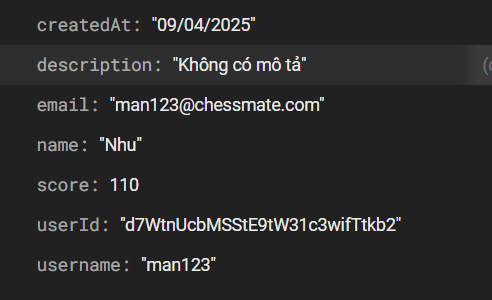
\includegraphics[width=0.9\textwidth]{img/user.png}
          \end{center}
    \item \textbf{friends:} quản lý mối quan hệ bạn bè
          \begin{center}
              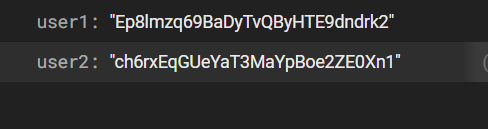
\includegraphics[width=0.9\textwidth]{img/friend.png}
          \end{center}
     \item \textbf{friends:} quản lý yêu cầu kết bạn
          \begin{center}
              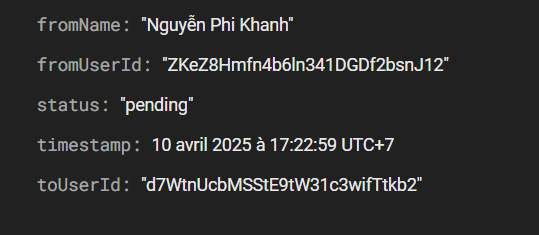
\includegraphics[width=0.9\textwidth]{img/friend_request.png}
          \end{center}
    \item \textbf{matches:} lưu thông tin các trận đấu
          \begin{center}
              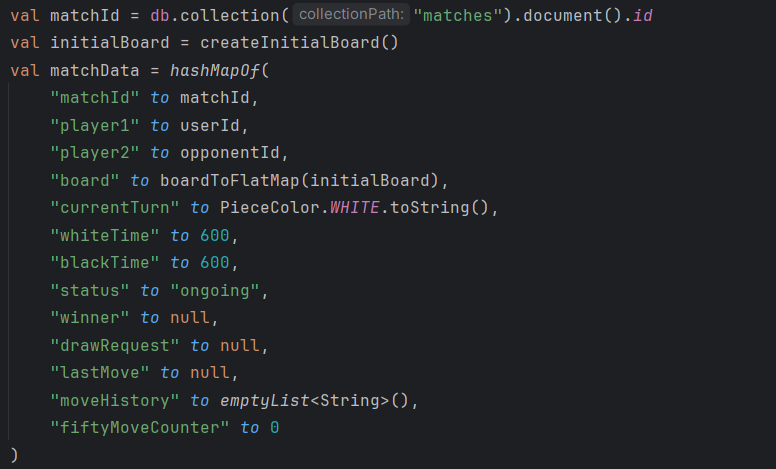
\includegraphics[width=0.9\textwidth]{img/match.png}
          \end{center}
    \item \textbf{rankings:} danh sách xếp hạng người chơi, có thể cập nhật định kỳ hoặc theo sự kiện
\end{itemize}

\subsection*{3.4. Thiết kế thuật toán chơi với AI}
\addcontentsline{toc}{subsection}{3.4. Thiết kế thuật toán chơi với AI}

\justify
\noindent Ứng dụng ChessMate tích hợp một chiến lược trí tuệ nhân tạo (AI) cơ bản để người dùng có thể chơi cờ vua với máy. Thuật toán này được triển khai trong phương thức \texttt{findBestMove()} của lớp \texttt{ChessViewModel}. Mục tiêu chính của thuật toán là tự động đưa ra nước đi cho quân Đen dựa trên trạng thái hiện tại của bàn cờ, ưu tiên việc bắt quân của đối phương. Dưới đây là phân tích chi tiết về cách thuật toán này hoạt động:

\subsubsection*{3.4.1. Xác định tất cả các nước đi hợp lệ}
\addcontentsline{toc}{subsubsection}{3.4.1. Xác định tất cả các nước đi hợp lệ}

\noindent Bước đầu tiên trong quá trình ra quyết định của AI là xác định tất cả các nước đi hợp lệ mà quân Đen có thể thực hiện trong lượt hiện tại. Điều này được thực hiện bởi phương thức \texttt{getAllMoves(PieceColor.BLACK)}. Phương thức này hoạt động theo các bước sau:
\begin{enumerate}[label=(\roman*)]
    \item Duyệt qua tất cả 64 ô trên bàn cờ, từ hàng 0 đến 7 và cột 0 đến 7.
    \item Tại mỗi ô, thuật toán kiểm tra xem có quân cờ nào đang đứng tại ô đó hay không và liệu quân cờ đó có phải là quân Đen hay không (có màu \texttt{PieceColor.BLACK}).
    \item Nếu tìm thấy một quân Đen, thuật toán sẽ gọi phương thức \texttt{game.selectPiece(row, col)} với vị trí hiện tại của quân cờ. Phương thức này (trong lớp \texttt{ChessGame}) sẽ trả về một danh sách các đối tượng \texttt{Move}, mỗi đối tượng chứa thông tin về một nước đi hợp lệ từ vị trí đã chọn, bao gồm cả vị trí đích (\texttt{position}).
    \item Đối với mỗi nước đi hợp lệ (\texttt{Move}), thuật toán sẽ tạo một cặp \texttt{Pair<Position, Position>}, với phần tử đầu tiên là vị trí hiện tại của quân cờ (vị trí đi) và phần tử thứ hai là vị trí đích của nước đi (\texttt{move.position}).
    \item Tất cả các cặp nước đi hợp lệ này sẽ được thêm vào một danh sách (\texttt{allMoves}).
    \item Cuối cùng, phương thức \texttt{getAllMoves()} trả về danh sách đầy đủ tất cả các nước đi hợp lệ mà quân Đen có thể thực hiện.
\end{enumerate}

\subsubsection*{3.4.2. Đánh giá và lựa chọn nước đi tốt nhất}
\addcontentsline{toc}{subsubsection}{3.4.2. Đánh giá và lựa chọn nước đi tốt nhất}

\noindent Sau khi đã có danh sách tất cả các nước đi hợp lệ, thuật toán sẽ tiến hành đánh giá từng nước đi để chọn ra nước đi tốt nhất dựa trên tiêu chí ưu tiên bắt quân của đối phương (quân Trắng). Quá trình này được thực hiện trong phương thức \texttt{findBestMove()}:
\begin{enumerate}[label=(\roman*)]
    \item Khởi tạo biến theo dõi nước đi tốt nhất: Thuật toán khởi tạo một biến \texttt{bestMove} để lưu trữ nước đi tốt nhất tìm được (ban đầu là \texttt{null}) và một biến \texttt{bestCaptureValue} để lưu trữ giá trị của quân cờ bị bắt trong nước đi tốt nhất (ban đầu là -1).
    \item Duyệt qua tất cả các nước đi hợp lệ: Thuật toán lặp qua từng cặp nước đi (\texttt{move}) trong danh sách \texttt{allMoves}. Mỗi cặp \texttt{move} chứa vị trí đi (\texttt{from}) và vị trí đến (\texttt{to}).
    \item Kiểm tra khả năng bắt quân: Đối với mỗi nước đi, thuật toán kiểm tra xem tại vị trí đích (\texttt{to.row}, \texttt{to.col}) có quân cờ nào của đối phương (quân Trắng, có màu \texttt{PieceColor.WHITE}) đang đứng hay không bằng cách gọi phương thức \texttt{game.getPieceAt(to.row, to.col)}.
    \item Tính giá trị của quân bị bắt (nếu có): Nếu một quân Trắng bị bắt, thuật toán sẽ xác định loại quân đó (\texttt{piece.type}) và gán cho nó một giá trị điểm số nhất định:
    \begin{itemize}[label=$\cdot$]
        \item Tốt (\texttt{PieceType.PAWN}): 1 điểm
        \item Mã (\texttt{PieceType.KNIGHT}): 3 điểm
        \item Tượng (\texttt{PieceType.BISHOP}): 3 điểm
        \item Xe (\texttt{PieceType.ROOK}): 5 điểm
        \item Hậu (\texttt{PieceType.QUEEN}): 9 điểm
        \item Vua (\texttt{PieceType.KING}): 100 điểm
    \end{itemize}
    \item **Cập nhật nước đi tốt nhất:** Nếu giá trị của quân bị bắt (\texttt{captureValue}) lớn hơn giá trị tốt nhất đã tìm thấy (\texttt{bestCaptureValue}), thuật toán sẽ cập nhật \texttt{bestCaptureValue} và lưu trữ nước đi hiện tại (\texttt{move}) vào biến \texttt{bestMove}.
    \item Lựa chọn ngẫu nhiên nếu không có nước đi bắt quân: Nếu sau khi duyệt tất cả các nước đi mà \texttt{bestMove} vẫn là \texttt{null}, thuật toán sẽ chọn một nước đi ngẫu nhiên từ danh sách \texttt{allMoves}.
    \item Trả về nước đi tốt nhất: Cuối cùng, phương thức \texttt{findBestMove()} trả về cặp \texttt{Pair<Position, Position>} đại diện cho nước đi được chọn.
\end{enumerate}

\subsubsection*{3.4.3. Thực hiện nước đi của AI}
\addcontentsline{toc}{subsubsection}{3.4.3. Thực hiện nước đi của AI }

\noindent Khi phương thức \texttt{findBestMove()} trả về một nước đi, phương thức \texttt{triggerAIMove()} sẽ thực hiện nước đi đó trên bàn cờ, cập nhật trạng thái trò chơi và xử lý trường hợp phong cấp tốt (nếu có).

\subsubsection*{3.4.4. Nhận xét về thuật toán}
\addcontentsline{toc}{subsubsection}{3.4.4. Nhận xét về thuật toán}

\noindent Thuật toán AI được sử dụng trong ChessMate là một chiến lược tham lam cơ bản, tập trung vào việc bắt quân đối phương. Mặc dù đơn giản, nó cung cấp một cơ chế để AI thực hiện các nước đi hợp lệ. Các cải tiến trong tương lai có thể bao gồm việc tích hợp các thuật toán phức tạp hơn để nâng cao khả năng chiến lược của AI.

\subsection*{3.5. Luồng hoạt động chính} % Heading 2 
\addcontentsline{toc}{subsection}{3.5. Luồng hoạt động chính}

\subsubsection*{3.5.1. Luồng chơi online} % Heading 3
\addcontentsline{toc}{subsubsection}{3.5.1. Luồng chơi online}


\begin{itemize}[label=·]
    \item Người dùng bấm "Chơi Online"
    \item Hệ thống kiểm tra phòng đang chờ
    \item Nếu có, ghép người chơi vào phòng đó; nếu không, tạo phòng mới
    \item Hai người chơi thi đấu theo lượt
    \item Khi ván đấu kết thúc, hệ thống cập nhật kết quả, lịch sử trận đấu, và điểm xếp hạng
\end{itemize}

\subsubsection*{3.5.2. Luồng thêm bạn} % Heading 3 
\addcontentsline{toc}{subsubsection}{3.5.2. Luồng thêm bạn}


\begin{itemize}[label=·]
    \item Người dùng tìm kiếm tên người chơi
    \item Gửi lời mời kết bạn
    \item Người nhận xác nhận lời mời
    \item Hệ thống cập nhật mối quan hệ trong collection friends
\end{itemize}


\section*{\centering \textbf{CHƯƠNG 4: KẾT QUẢ VÀ HƯỚNG PHÁT TRIỂN}} % Heading 1 
\addcontentsline{toc}{section}{CHƯƠNG 4: KẾT QUẢ VÀ HƯỚNG PHÁT TRIỂN}

\subsection*{4.1. Kết quả đạt được} % Heading 2 
\addcontentsline{toc}{subsection}{4.1. Kết quả đạt được}

\justify
\noindent Sau một quá trình tìm tòi, nghiên cứu, thiết kế và triển khai, ứng dụng ChessMate đã được xây dựng thành công và hoàn thiện các chức năng chính như sau:

\paragraph{\textbf{Chức năng xác thực người dùng:}} % Paragraph
\begin{itemize}[label=·]
    \item Đăng nhập bằng tài khoản email và mật khẩu thông qua Firebase Authentication.
    \item Đăng nhập nhanh bằng tài khoản Google (Google Sign-In).
    \item Đăng ký tài khoản mới và xác minh đầu vào cơ bản.
    \item Chức năng “Quên mật khẩu” giúp người dùng khôi phục mật khẩu thông qua email.
\end{itemize}

\paragraph{\textbf{Chức năng chơi cờ:}} % Paragraph 
\begin{itemize}[label=·]
    \item Chơi với bạn bè: Hai người cùng chơi trực tiếp trên một thiết bị.
    \item Chơi với AI: Ứng dụng tích hợp thuật toán để xây dựng AI có khả năng chơi cờ với nhiều mức độ khó khác nhau.
    \item Chơi online: Người dùng có thể ghép trận ngẫu nhiên và chơi cờ trực tuyến với người chơi khác.
    \item Chức năng chat với đối thủ khi chơi ghép trực tuyến.
\end{itemize}

\paragraph{\textbf{Chức năng mạng xã hội:}} % Paragraph 
\begin{itemize}[label=·]
    \item Gửi lời mời kết bạn, chấp nhận, từ chối lời mời.
    \item Danh sách bạn bè có thể xem thông tin, gửi lời mời chơi.
    \item Tìm kiếm người chơi theo tên.
    \item Chức năng chat với bạn bè.
\end{itemize}

\paragraph{\textbf{Chức năng quản lý người dùng:}} % Paragraph 
\begin{itemize}[label=·]
    \item Xem và chỉnh sửa thông tin cá nhân (tên hiển thị, mô tả...).
    \item Xem thông tin chi tiết của bạn bè và đối thủ đã từng chơi cùng.
\end{itemize}

\paragraph{\textbf{Lịch sử và thống kê:}} % Paragraph 
\begin{itemize}[label=·]
    \item Lưu trữ lịch sử các ván đấu, bao gồm thời gian, kết quả, và các nước đi.
    \item Hiển thị lại bàn cờ và diễn biến trận đấu.
\end{itemize}

\paragraph{\textbf{Mô hình kiến trúc MVVM:}} % Paragraph 
\noindent Ứng dụng được xây dựng theo mô hình MVVM (Model - View - ViewModel) giúp phân tách rõ ràng giữa giao diện, logic xử lý và dữ liệu, tăng khả năng bảo trì, mở rộng và tái sử dụng code.

\paragraph{\textbf{Công nghệ sử dụng:}} % Paragraph 
\begin{itemize}[label=·]
    \item \textbf{Ngôn ngữ lập trình:} Kotlin
    \item \textbf{Giao diện:} Jetpack Compose – giúp viết UI bằng code, dễ tùy biến và hiện đại.
    \item \textbf{Cơ sở dữ liệu:} Firestore – lưu trữ thông tin người dùng, bạn bè, lịch sử trận đấu.
    \item \textbf{Xác thực:} Firebase Authentication
\end{itemize}

\subsection*{4.2. Hạn chế} % Heading 2 
\addcontentsline{toc}{subsection}{4.2. Hạn chế}

\justify
\noindent Dù ứng dụng đã đạt được nhiều kết quả tích cực, vẫn còn một số điểm hạn chế cần cải thiện:
\begin{itemize}[label=·]
    \item Cần cải thiện hệ thống đánh giá AI để hỗ trợ nhiều cấp độ khó khăn hơn:
    \begin{itemize}[label=$\circ$]
        \item Hệ thống đánh giá AI hiện tại mới chỉ được xây dựng dựa trên một thuật toán cơ bản, tập trung chủ yếu vào việc tối ưu hóa lợi thế vật chất bằng cách ưu tiên các nước đi bắt quân của đối phương. Mặc dù cách tiếp cận này cho phép AI đưa ra các nước đi hợp lệ và tạo ra một đối thủ ở mức độ nhập môn, nhưng nó tồn tại nhiều hạn chế.
        \item Thuật toán hiện tại thiếu khả năng xem xét các yếu tố chiến lược phức tạp và sâu sắc hơn, vốn là nền tảng của một ván cờ vua ở trình độ cao. Các yếu tố như kiểm soát trung tâm bàn cờ, sự phát triển hài hòa của các quân cờ, mức độ an toàn của Vua, cấu trúc tốt vững chắc, và khả năng tạo ra các mối đe dọa chiếu hết tiềm năng hiện chưa được đánh giá một cách đầy đủ.
        \item Do sự đơn giản trong logic đánh giá, AI hiện tại dễ dàng bị đánh bại bởi những người chơi có kinh nghiệm, những người có khả năng nhìn nhận ván cờ ở một tầm chiến lược cao hơn và có thể khai thác những điểm yếu trong cách AI lựa chọn nước đi. AI thiếu khả năng lập kế hoạch dài hạn và không có khả năng đánh giá toàn diện các vị trí phức tạp trên bàn cờ.
    \end{itemize}
    \item Tính năng chơi online đôi khi bị chậm do phụ thuộc vào tốc độ kết nối mạng và quá trình đồng bộ Firestore.
    \item Giao diện chưa tối ưu hoàn toàn cho tất cả kích thước màn hình.
    \item Chưa có tính năng sửa ảnh avatar.
    \item Chưa có tính năng xếp hạng người chơi dựa trên số trận thắng/thua và thời gian hoạt động.
    \item Bổ sung hiệu ứng âm thanh tương tác trong quá trình chơi và di chuyển quân cờ:
    \begin{itemize}[label=$\circ$]
        \item Tích hợp các hiệu ứng âm thanh sống động và phù hợp với từng hành động trong trò chơi, chẳng hạn như âm thanh khi người chơi thực hiện một nước đi, âm thanh khi quân cờ bị bắt, hoặc các hiệu ứng âm thanh đặc biệt cho các sự kiện quan trọng như chiếu tướng hoặc hết cờ.
        \item Cung cấp tùy chọn cho người dùng điều chỉnh âm lượng hoặc tắt/bật hiệu ứng âm thanh theo sở thích cá nhân, tạo sự thoải mái và tùy biến trong trải nghiệm chơi.
        \item Nghiên cứu và lựa chọn các hiệu ứng âm thanh chất lượng cao, đảm bảo tính thẩm mỹ và không gây xao nhãng cho người chơi, góp phần tăng thêm sự hấp dẫn và tính chân thực cho ứng dụng.
    \end{itemize}
\end{itemize}

\subsection*{4.3. Hướng phát triển} % Heading 2 
\addcontentsline{toc}{subsection}{4.3. Hướng phát triển}

\justify
\noindent Trong thời gian tới, ứng dụng ChessMate có thể được nâng cấp với các tính năng mới và tối ưu như sau:

\paragraph{\textbf{Cải tiến hiệu năng:}} % Paragraph 
\begin{itemize}[label=·]
    \item Tối ưu tốc độ load dữ liệu từ Firestore.
    \item Sử dụng Cloud Functions để xử lý một số logic phía server.
    \item Sử dụng Firebase Storage để lưu trữ ảnh .
\end{itemize}

\paragraph{\textbf{Tính năng mở rộng:}} % Paragraph 
\begin{itemize}[label=$\cdot$]
    \item Hệ thống thành tích và huy hiệu cho người chơi:
    \begin{itemize}[label=$\circ$]
        \item Phát triển một hệ thống thành tích đa dạng, ghi nhận những cột mốc quan trọng và những chiến thắng ấn tượng của người chơi trong quá trình sử dụng ứng dụng.
        \item Thiết kế các huy hiệu độc đáo và có giá trị tượng trưng khác nhau, trao thưởng cho người chơi khi họ đạt được các thành tích nhất định, khuyến khích sự tham gia tích cực và tạo động lực để người chơi tiếp tục rèn luyện và nâng cao kỹ năng.
        \item Cho phép người chơi hiển thị các thành tích và huy hiệu đã đạt được trên hồ sơ cá nhân, tạo điểm nhấn và thể hiện đẳng cấp của họ trong cộng đồng người chơi ChessMate.
    \end{itemize}
    \item Thêm nhiều cấp độ AI và nâng cao trí tuệ nhân tạo bằng các kỹ thuật Machine Learning:
    \begin{itemize}[label=$\circ$]
        \item Mở rộng số lượng cấp độ khó của AI, từ cơ bản đến nâng cao, nhằm đáp ứng nhu cầu luyện tập của người chơi ở mọi trình độ.
        \item Thay thế thuật toán AI hiện tại bằng các thuật toán tìm kiếm cây trò chơi tiên tiến như \textbf{Minimax} và \textbf{Alpha-Beta Pruning} để cải thiện khả năng dự đoán và lựa chọn nước đi của AI. Các thuật toán này sẽ cho phép AI "nhìn xa" hơn trong các tình huống trên bàn cờ và đưa ra các quyết định chiến lược phức tạp hơn.
        \item Xây dựng một \textbf{Hàm đánh giá (Evaluation Function)} tinh vi, có khả năng định lượng giá trị của một trạng thái bàn cờ dựa trên nhiều yếu tố chiến lược quan trọng như giá trị vật chất, kiểm soát trung tâm, sự phát triển quân, cấu trúc tốt, an toàn của Vua và tính di động của quân. Việc tối ưu hóa hàm đánh giá sẽ giúp AI đưa ra những nhận định chính xác hơn về tình hình ván cờ.
        \item Nghiên cứu và ứng dụng các kỹ thuật \textbf{Học máy (Machine Learning)}, đặc biệt là việc huấn luyện \textbf{mạng nơ-ron sâu (Deep Neural Network)} trên một lượng lớn dữ liệu các ván cờ chất lượng cao. Mục tiêu là giúp AI học hỏi các mẫu hình chiến lược phức tạp và đưa ra những nước đi tối ưu dựa trên kinh nghiệm đã học được, vượt xa khả năng được lập trình thủ công. Việc tích hợp học máy có tiềm năng tạo ra một AI không chỉ mạnh mẽ mà còn có khả năng thích ứng với phong cách chơi của từng người dùng.
    \end{itemize}
\end{itemize}

\paragraph{\textbf{Tích hợp dịch vụ bên ngoài:}} % Paragraph
\begin{itemize}[label=·]
    \item Tích hợp Firebase Cloud Messaging để gửi thông báo khi có lời mời kết bạn, thách đấu...
    \item Đồng bộ tài khoản và xếp hạng qua Google Play Games.
\end{itemize}

\subsection*{4.4. Kết quả học tập đạt được} % Heading 2
\addcontentsline{toc}{subsection}{4.4. Kết quả học tập đạt được}

\justify
\noindent Thông qua quá trình thực hiện đồ án, nhóm đã học được và củng cố nhiều kiến thức, bao gồm:
\begin{itemize}[label=·]
    \item Thành thạo hơn trong sử dụng Kotlin và Jetpack Compose để phát triển ứng dụng Android hiện đại.
    \item Hiểu rõ về mô hình kiến trúc MVVM trong thực tế.
    \item Biết cách tích hợp Firebase (Authentication, Firestore, Storage) vào ứng dụng Android.
    \item Có thêm kinh nghiệm về thuật toán AI và xử lý logic cờ vua.
    \item Rèn luyện kỹ năng làm việc nhóm, chia nhỏ task và tổ chức tiến độ hợp lý.
\end{itemize}

\newpage

\section*{\centering \textbf{KẾT LUẬN}} % Heading 1 căn giữa, in đậm
\addcontentsline{toc}{section}{KẾT LUẬN}

\justify
\noindent Sau một khoảng thời gian tìm hiểu, nghiên cứu và thực hiện, nhóm đã hoàn thành ứng dụng ChessMate – một ứng dụng chơi cờ vua hiện đại, tiện lợi trên nền tảng Android. Ứng dụng được xây dựng bằng ngôn ngữ Kotlin, sử dụng Jetpack Compose cho giao diện và Firebase làm nền tảng backend, đáp ứng đầy đủ các chức năng như: chơi với bạn, chơi với AI, ghép trận online, quản lý tài khoản, bạn bè, và lưu lịch sử trận đấu.

\noindent Thông qua đồ án này, nhóm không chỉ củng cố kiến thức về lập trình Android và mô hình kiến trúc MVVM mà còn học được cách giải quyết vấn đề thực tế, thiết kế logic hợp lý và phối hợp làm việc nhóm hiệu quả. Đặc biệt, việc xây dựng AI để chơi cờ là một thử thách thú vị và giúp nhóm hiểu sâu hơn về thuật toán Minimax và cách tối ưu nó.

\noindent Tuy còn một số hạn chế cần cải thiện, nhưng kết quả hiện tại là bước đệm vững chắc để nhóm có thể tiếp tục nâng cấp và phát triển ứng dụng trong tương lai. Đây cũng là một trải nghiệm học tập rất đáng nhớ và hữu ích trong hành trình trở thành lập trình viên chuyên nghiệp.

\noindent Nhóm xin chân thành cảm ơn thầy Trương Quang Tuấn đã tận tình hướng dẫn, góp ý trong suốt quá trình thực hiện đồ án này.

\newpage % Bắt đầu trang mới cho Tài liệu tham khảo

\section*{\centering \textbf{TÀI LIỆU THAM KHẢO}} % Heading 1, căn giữa, in đậm
\addcontentsline{toc}{section}{TÀI LIỆU THAM KHẢO}


\begin{thebibliography}{99} % Sử dụng môi trường thebibliography với nhãn số tối đa là 99

    \bibitem{android_kotlin}
    Android Developers. \textit{Kotlin on Android}.
    \href{https://developer.android.com/kotlin}{\nolinkurl{https://developer.android.com/kotlin}}
    (Truy cập ngày 15 tháng 3 năm 2025).

    \bibitem{jetpack_compose}
    Android Developers. \textit{Jetpack Compose}.
    \href{https://developer.android.com/jetpack/compose}{\nolinkurl{https://developer.android.com/jetpack/compose}}
    (Truy cập ngày 18 tháng 3 năm 2025).

    \bibitem{firebase_docs}
    Firebase Documentation.
    \href{https://firebase.google.com/docs}{\nolinkurl{https://firebase.google.com/docs}}
    (Truy cập ngày 25 tháng 3 năm 2025).

    \bibitem{mvvm_android}
    Google Developers. \textit{Guide to app architecture}.
    \href{https://developer.android.com/topic/architecture}{\nolinkurl{https://developer.android.com/topic/architecture}}
    (Truy cập ngày 01 tháng 4 năm 2025).

    \bibitem{chess_standard}
    FIDE. \textit{Laws of Chess}.
    \href{https://handbook.fide.com/chapter/E012023}{\nolinkurl{https://handbook.fide.com/chapter/E012023}}
    (Truy cập ngày 10 tháng 4 năm 2025).


\end{thebibliography}

\end{document}